\documentclass[margin=2cm]{standalone}

\usepackage{tikz}
\usetikzlibrary{positioning}

\def\myscale{1}

\begin{document}

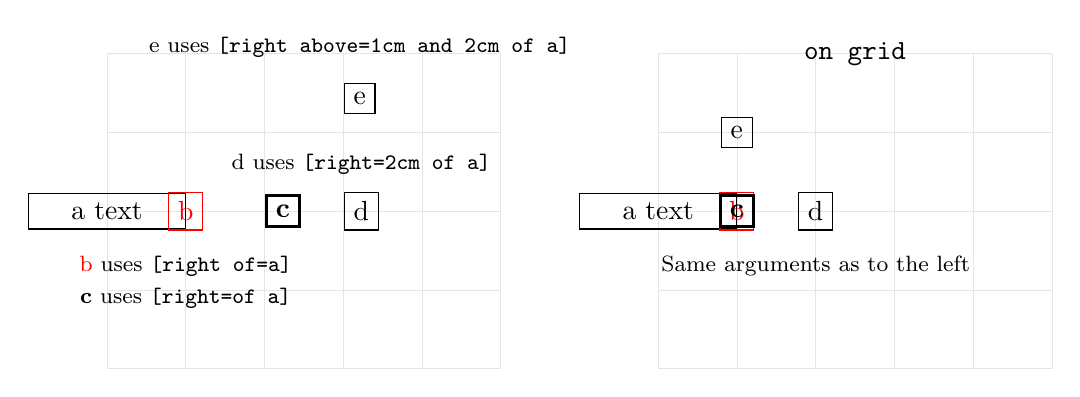
\begin{tikzpicture}[node distance=1cm, scale=\myscale, every node/.style={scale=1*\myscale}, node distance=\myscale cm]
    \draw[help lines,step=10mm,gray!20] (0,0) grid (5,4);


    % Nodes
    \node (a) at (0,2) [draw, minimum width=2cm] {a text};

    \node (b) [right of=a] [draw,red] {b};
        
    \node (c) [right=of a] [draw,very thick] {\textbf{c}};
    \node (d) [right=2cm of a] [draw] {d};
    \node (e) [above right=1cm and 2cm of a] [draw] {e};
    
    
    % Descriptive text
    \node (b text) [below=2mm of b] {\footnotesize \textcolor{red}{b} uses \texttt{[right of=a]}};
    \node [below=-1mm of b text] {\footnotesize \textbf{c} uses \texttt{[right=of a]}};
    \node [above=1mmof d] {\footnotesize d uses \texttt{[right=2cm of a]}};
    \node [above=2mm of e] {\footnotesize e uses \texttt{[right above=1cm and 2cm of a]}};

    % Same but with 'on grid'
    \begin{scope}[xshift=7cm, on grid]
        \draw[help lines,step=10mm,gray!20] (0,0) grid (5,4);
        \node at (2.5,4) {\texttt{on grid}};

        \node (a) at (0,2) [draw, minimum width=2cm] {a text};
        \node (b) [right of=a] [draw,red] {b};
        
        \node (c) [right=of a] [draw,very thick] {\textbf{c}};
        \node (d) [right=2cm of a] [draw] {d};
        \node (e) [above right=1cm and 1cm of a] [draw] {e};

        \node [below=7mm of d] {\footnotesize Same arguments as to the left};
    \end{scope}
\end{tikzpicture}

\end{document}